Este capítulo tem como objetivo apresentar uma base teórica dos conceitos necessários para o entendimento das demais seções deste trabalho. Primeiramente, será explorado o que é aprendizado de máquina e algumas classificações úteis. Subsequentemente, será explicado os conceitos básicos por trás de cada um dos modelos utilizados nesse trabalho. Para a explicação de alguns modelos, será necessária uma elucidação prévia de alguns conceitos fundamentais por trás de seu funcionamento. Será explicado o conceito de árvores de regressão para depois ser explicado o funcionamento de \textit{\acrshort{RF}} e, posteriormente, será explicado o que é uma \textit{\acrshort{RNN}}, para que seja possível explicar como funcionam os modelos \textit{\acrshort{LSTM}} e \textit{\acrshort{GRU}}.

\section{Aprendizado de Máquina}

Segundo Murphy et. al. \cite{murphy2012machine}, aprendizado de máquina é definida como um conjunto de técnicas que encontram, automaticamente, padrões em um dado conjunto de dados, que pode estar imperfeito ou incompleto para determinado problema. Também é dito que a aprendizado de máquina utiliza os padrões descobertos para tentar prever ou decidir algo. Para realizar tal tarefa, existe uma variedade de técnicas que podem ser classificadas como aprendizagem supervisionadas, não-supervisionadas, ou por reforço. A classificação se dá pela maneira como o algoritmo utilizado aprende o padrão dos dados.

Técnicas de aprendizagem não-supervisionadas são aquelas que buscam, a partir de um conjunto de dados(\(\set{x_i \mid 1\leq i\leq N}\)) utilizado como entrada do algoritmo, identificar a que grupo pertence um certo dado sem nenhum tipo de comentário sobre suas identificações. Técnicas de aprendizagem por reforço são aquelas que tentam aprender a partir da tentativa e erro, dado que o problema forneça recompensa e/ou punição para certas ações. Esse tipo de técnica pode ser usada para ensinar um robô a jogar \textit{Tetris}, por exemplo. Técnicas de aprendizagem supervisionadas são aquelas que tentam mapear uma entrada a uma classe correspondente (\(f(x) = y\)). Normalmente, essas técnicas utilizam de um conjunto de pares de entrada e classe (\(\set{(x_i, y_i) \mid 1\leq i\leq N}\)) para aprender a fazer o mapeamento, isto é, utilizam um conjunto de treinamento para aprender. Caso a classe seja do tipo nominal, a técnica é do sub-tipo classificador e caso seja do tipo ordinal, a técnica é do sub-tipo regressor.

Além disso, as técnicas de aprendizado de máquina também podem ser classificadas de acordo com as suposições feitas por elas sobre o conjunto de dados utilizados. Essas classificações podem ser paramétricas ou não-paramétricas. Técnicas paramétricas dispõe de um número fixo de parâmetros para tentar descrever os dados, supondo assim que os dados seguem uma distribuição específica. Um exemplo de modelo paramétrico seria a regressão linear, que utiliza uma equação com parâmetros fixos para traçar uma reta que melhor representa a distribuição dos dados. Já modelos não-paramétricos possuem um número variável de parâmetros que dependem dos dados utilizados. Desse modo, não é feita uma suposição de que existe uma distribuição específica nos dados. Modelos paramétricos levam a vantagem na questão de velocidade de treinamento, porém perdem na questão flexibilidade. A escolha de qual tipo utilizar depende muito do formato dos dados do problema e do seu tamanho, dentre outros fatores.

\section{Árvores de Regressão}

De acordo com Trevor Hastie et. al. \cite{hastie2005elements}, árvore é uma técnica que pode ser utilizado para aprendizado de máquina supervisionada no qual pode ser usado tanto para classificação (árvores de decisão), quanto para regressão (árvores de regressão). Basicamente, árvores dividem o espaço de características utilizando de regras.

Árvores utilizam de um algoritmo guloso. Isto é, os melhores resultados locais fazem parte do melhor resultado global. Inicialmente, o algoritmo escolhe uma das características e define uma regra a partir da mesma. Assim, dividindo os dados em dois conjuntos. Por exemplo, considere que uma característica seja idade, uma regra possível seria \texttt{Idade \(\leq\) 40}. Seguindo esta regra o algoritmo divide os dados. Para os conjuntos resultantes, é definido uma nova regra e isso acontece sucessivamente até que não seja mais possível dividir os dados.

Existem algumas formas de decidir qual o melhor par, característica e regra, para um conjunto de dados. Uma das formas possíveis seria: para cada uma das características, ou conjunto de características, determina-se a melhor regra que divide o conjunto de dados no nó atual e compara essas regras para determinar qual o melhor par. Desta forma, é possível comparar os pares resultantes com um custo aceitável. A comparação entre os pares pode ser feita de diversas formas, para classificação pode ser usado o \textit{Gini Index} e para regressão pode ser usado a Soma do Erros Quadráticos. Uma vez construída a árvore, para utilizá-la basta percorrê-la seguindo as regras já definidas, assim como mostrado na Figura \ref{figure:tree}.

É importante notar a grande flexibilidade desse modelo de se ajustar ao conjunto de dados, isto é, árvores podem sofrer com o problema do sobre-ajuste (\textit{overfitting}). Por exemplo, é possível que o modelo tenha em cada folha da árvore um elemento do conjunto de dados. Para resolver este problema, é necessário controlar certos aspectos da construção da árvore, como a sua altura máxima, ou o limite mínimo de tamanho necessário para se dividir o conjunto. Trevor Hastie et. al. \cite{hastie2005elements} sugerem utilizar o segundo método, seguido de uma redução da árvore resultante, porém, dependendo dos dados, podem vir a existir modelos de construção melhores.
 
 \begin{figure}[htbp]
    \centering
    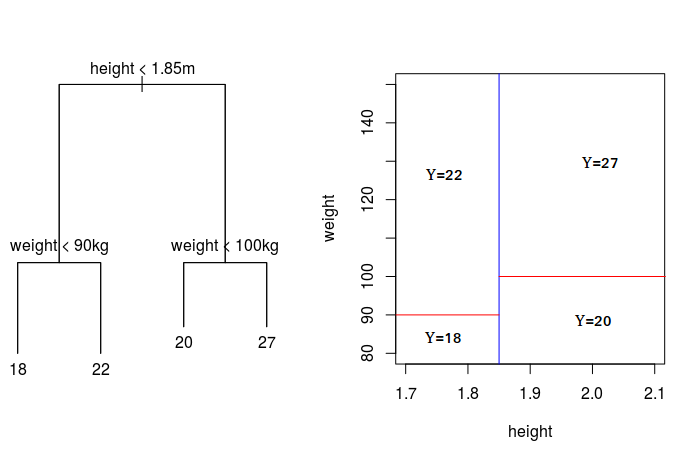
\includegraphics[scale=0.6]{monography/img/models/regression_tree.png}
    \label{figure:tree}
    \caption[Árvore de Regressão Dividindo o Espaço de Resposta]{Árvore de Regressão Dividindo o Espaço de Resposta\footnotemark}
\end{figure}

\footnotetext{\url{https://www.r-bloggers.com/how-random-forests-improve-simple-regression-trees/}}

\section{\textit{\acrfull{RF}}}

Desenvolvido por Leo Breiman em \textit{Random Forest} \cite{Breiman:2001:RF:570181.570182}, \textit{\acrshort{RF}} é um método de aprendizado de máquina utilizado tanto para classificação quanto para regressão. Segundo o autor, o método é uma combinação de árvores, de decisões ou regressão, onde cada árvore depende de uma amostra aleatória, sendo esta amostra independente do conjunto de dados. Além disso, todas as árvores devem possuir a mesma distribuição. 

A construção das árvores é feita utilizando o método \textit{Bagging} (\textit{\textbf{B}ootstrap \textbf{Agg}regation}), também criado por Leo Breiman em \textit{Bagging Predictors} \cite{Breiman:1996:BP:231986.231989}. Este método gera várias versões de um mesmo modelo e agrega os resultados dos mesmos. As versões do modelo utilizam amostras do conjunto de dados selecionadas aleatoriamente, mas com a mesma distribuição.

\begin{figure}[htbp]
    \centering
    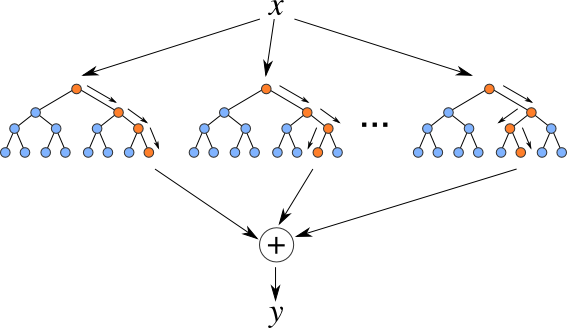
\includegraphics[scale=1.0]{monography/img/models/random_forest.png}
    \label{figure:random_forest}
    \caption[Representação do funcionamento de uma \textit{\acrshort{RF}}]{Representação do funcionamento de uma \textit{\acrshort{RF}}\footnotemark}
\end{figure}

\footnotetext{Imagem vinda da documentação da biblioteca Harp (\url{https://dsc-spidal.github.io/harp/docs/examples/rf/})}

Porém, diferente de \textit{Bagging}, \textit{\acrshort{RF}} utiliza mais uma técnica para diminuir o sobre-ajuste. Há uma modificação no algoritmo de criação das árvores de decisão limitando a quantidade de características (\textit{features}) do conjunto de dados que vai ser utilizada. O autor sugere limitar a quantidade de características (\textit{q}) para $ \sqrt{q} $, no caso de classificação, ou $ \frac{q}{3} $, no caso de regressão \cite{hastie2005elements}. Além disso, o autor também sugere, no artigo original, que, para selecionar a quantidade ideal de características deve-se utilizar de estimativas \textit{out-of-bag}, explicadas também no artigo.

Como \textit{\acrshort{RF}} é uma combinação de outros modelos de aprendizado de máquina, ela pode ser classificada como um Comitê de Máquinas (\textit{Ensemble Learning}). A forma como as respostas de cada uma das máquinas são combinadas depende do problema. Para classificação pode ser usado uma votação (voto da maioria) e para um problema de regressão pode ser usado uma média dos valores, assim como mostrado na Figura \ref{figure:random_forest}.

\section{\textit{\acrfull{SVM}}}

\textit{\acrshort{SVM}} foi criado originalmente por Vladimir Vapnik nos anos 60 e foi evoluindo até se tornar o que é hoje \cite{Smola03atutorial}. Essa técnica é não-paramétrica e supervisionada, sendo que a ideia básica por trás de seu funcionamento pode ser usada tanto para classificação quanto para regressão. Quando for utilizada para classificação, é chamado de \textit{\acrfull{SVC}} e quando é utilizado para regressão, é chamado de \textit{\acrfull{SVR}}. O nome deriva da técnica de enxergar as entradas (\(x_i\)) como vetores de atributos, onde somente alguns destes vetores servem para a solução final do problema, servindo de suporte.

\begin{figure}[htbp]
    \centering
    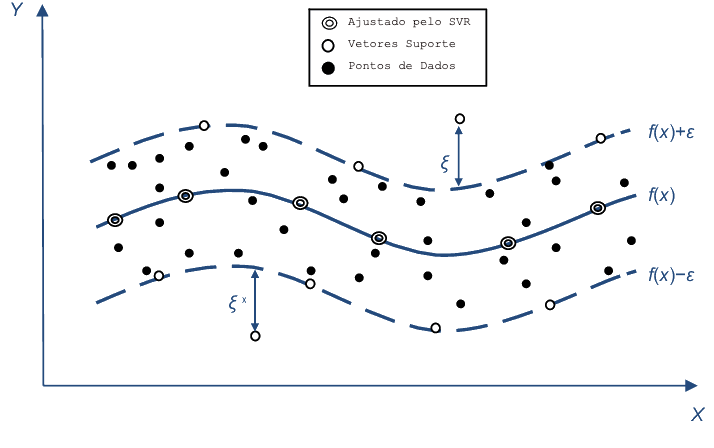
\includegraphics[scale=0.6]{monography/img/models/svr_example.png}
    \label{figure:support_vector_machine}
    \caption[Representação do funcionamento de uma \textit{\acrshort{SVM}}]{Representação do funcionamento de uma \textit{\acrshort{SVR}}\footnotemark}
\end{figure}

\footnotetext{Imagem baseada na Figura publicada por Saeid Shokri et. al. \cite{shokri_2015}}

No caso da \textit{\acrshort{SVR}}, tenta-se criar uma função \(f(x)\) de forma que se \(g(x)\) é a função que perfeitamente descreve o conjunto de dados e \(\epsilon\) seja a dimensão do erro, para todo \(f(x)\) \(\abs{g(x) - f(x)} \leq \epsilon \). Sendo assim, todos os pontos que estão dentro do ``tubo'' representam um erro esperado, assim como mostra a Figura \ref{figure:support_vector_machine}. Já os vetores de atributos que não estão dentro do tubo, nem estão servindo de suporte são utilizados para ajustar a função como erros. Vale notar que tanto para \textit{\acrshort{SVC}} quanto \textit{\acrshort{SVR}} é necessário que sejam determinados um \textit{Kernel} e uma constante de regulação (\(C\)) \cite{murphy2012machine}. Essa constante de regulação indica em quanto os erros serão penalizados. Se for baixo, erros não serão muito penalizados e se for alto os erros serão muito penalizados.

É importante notar que nem sempre é possível criar uma função que consiga se ajustar bem ao conjunto de dados. Para consertar esse problema, é feito uma mudança da dimensão dos vetores de atributos para outra dimensão que seja possível criar uma função que se ajuste melhor. Porém, mapear todo um conjunto de dados para outra representação do espaço é computacionalmente intenso. Nisso, entram as funções \textit{Kernel} que mapeiam dois pontos que pertencem a algum certo espaço para a distância deles em alguma outra representação desse espaço. Esse mapeamento é menos exigente computacionalmente, tornando então desnecessário mapear todo o conjunto de dados para a outra representação. Porém, mesmo com o \textit{Kernel}, \textit{\acrshort{SVM}} não escala muito bem para conjunto de dados muito grandes. \cite{chollet2018deep}

Mais especificamente esse truque é conhecido como \textit{Kernel Trick}, onde se substitui todas as multiplicações dos vetores de características (\(\langle x_i, x_j \rangle\)) por uma chamada do \textit{Kernel} (\(\kappa(x_i, x_j)\)) \cite{murphy2012machine}. Vale notar que alguns \textit{Kernels} possuem uma possibilidade de ajuste, permitindo ajustar o \textit{Kernel} ao conjunto de dados. \textit{Kernels} como o \textit{\acrfull{RBF}} podem ajustar a precisão (\(\gamma\)) que acaba determinando a influência dos \textit{support vectors} \cite{murphy2012machine}. Quanto menor o valor, maior a influência e vice versa. Valores baixos podem levar a uma função que não se ajusta muito ao conjunto de dados, prono a sub-ajuste (\textit{underfitting}). Já valores altos podem levar a uma função que se ajusta muito ao conjunto de dados, prono a sobre-ajuste.

\section{\textit{\acrfull{RNN}}}

\textit{\acrshort{RNN}} é uma classe de redes neurais artificiais na qual a arquitetura foi baseada nas conexões cíclicas do cérebro. Diferente das redes neurais comuns, \textit{\acrshort{RNN}}s possuem ciclos e laços iterativos que permitem guardar informação. \cite{alex2012} 

Ao se permitir guardar informações, é possível resolver uma outra classe de problemas, já que agora resultados passados podem influenciar o resultado atual \cite{alex2012}. Redes neurais comuns, ou do tipo \textit{feedforward}, utilizam apenas o seu estado atual para gerar o resultado. Estas conseguem resolver, por exemplo, problemas de classificação de imagens e até regressões. Porém, não lidam bem com problemas nos quais a resposta atual tem correlação com informações do passado. Um exemplo de problema que exige essa correlação seria a de tentar prever a próxima palavra de uma frase, ou tentar extrair um contexto de um documento. Segundo Mitchell et. al. \cite{Mitchell_1997}, para esse tipo de situação, {\acrshort{RNN}} são mais adequadas. Portanto, problemas onde os dados isolados não tem tanto significado quanto o conjunto inteiro exigem um conceito de memória, onde a utilização de \acrshort{RNN} é mais adequada.

Para simular esse efeito de memória, \textit{\acrshort{RNN}} dispõe de uma arquitetura onde a saída do nó anterior é utilizada como entrada no nó seguinte, juntamente com a entrada nova atual da rede (\(y_t = f(y_{t-1}, x_t)\)). Para passar estes valores de um nó para o outro, a \textit{\acrshort{RNN}} dispõe de um mecanismo chamado \textit{Hidden Layer}. Na Figura \ref{figure:rnn} é exemplificada a sua arquitetura quando desdobrada, onde o último resultado utiliza como entrada valores resultantes das execuções anteriores.

\begin{figure}[htbp]
    \centering
    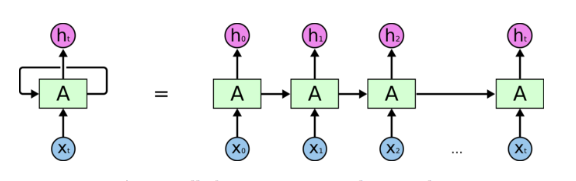
\includegraphics[scale=0.4]{monography/img/models/rnnExample.png}
    \label{figure:rnn}
    \caption[Representação simples do conceito de um RNN]{Representação simples do conceito de uma RNN \footnotemark}
\end{figure}

É importante notar que essa técnica possui limitações, como ser possível acessar apenas informações em uma direção. Por exemplo, em um contexto temporal, é possível apenas acessar o passado. Esta característica vai ao encontro com as características de problemas que envolvam séries temporais, mas podem não encaixar muito bem em outros tipos de problemas que possam exigir acesso de informações de maneira bidirecional \cite{alex2012}. Outra falha é a incapacidade de armazenar informações por um longo período de tempo \cite{hochreiter2001gradient}. 

Além das características já citadas, também é válido dizer que \textit{\acrshort{RNN}s} são muito difíceis de treinar, devido a um problema chamado \textit{Vanishing Gradient}. Esse problema se refere ao decaimento do erro, utilizado para ajustar os pesos da rede, em escala exponencial. O \textit{Vanishing Gradient} faz com que o o erro desapareça, tornando difícil a convergência da rede. \cite{doi:10.1162/neco.1997.9.8.1735}

\section{\textit{\acrfull{LSTM}}}

\textit{\acrshort{LSTM}} é um método proposto pela primeira vez por Sepp Hochreiter e Jurgen Schmidhuber \cite{doi:10.1162/neco.1997.9.8.1735}. A técnica foi criada como uma solução para o problema do \textit{Vanishing Gradient}, que ocorre em \textit{\acrshort{RNN}}'s \cite{doi:10.1162/neco.1997.9.8.1735}. Isto é, \textit{\acrfull{BPTT}} e \textit{\acrfull{RTRL}}, técnicas usadas para propagar o erro na rede, podiam ou decair a ponto de não ter efeito em algumas camadas da \textit{\acrshort{RNN}} ou ficarem com erros exorbitantes, o que dificulta o aprendizado. 

\begin{figure}[htbp]
    \centering
    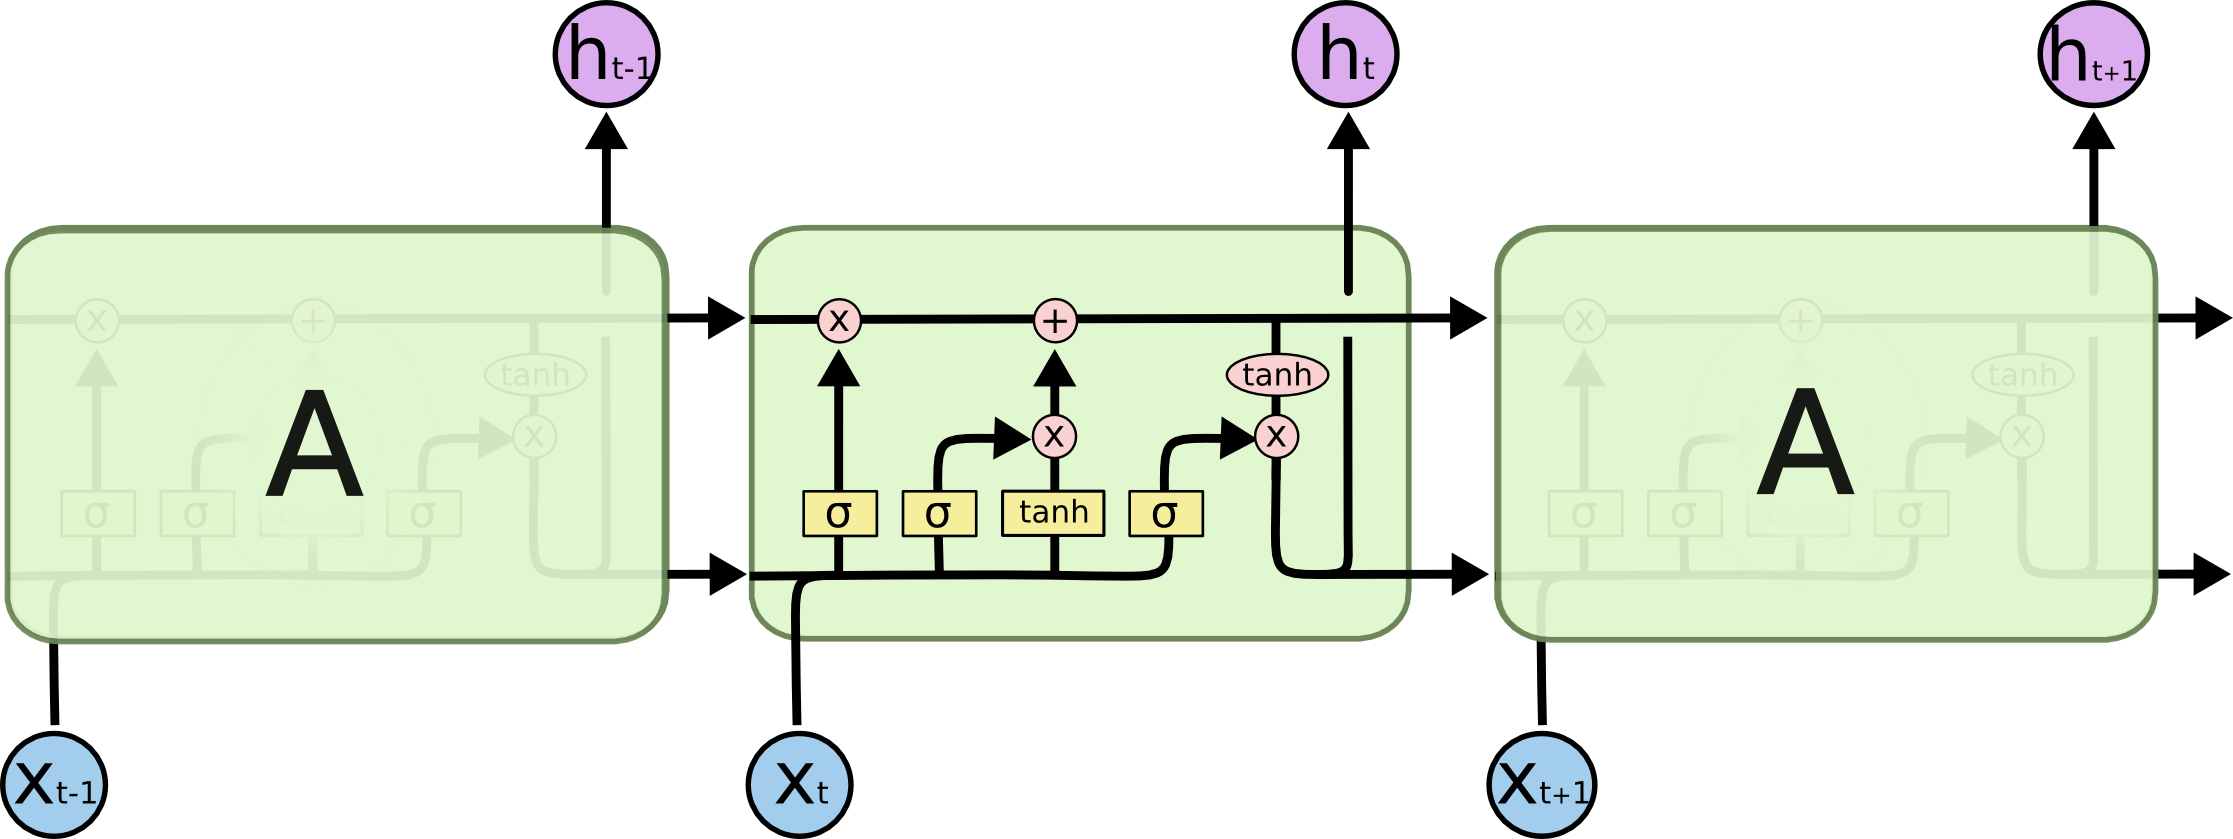
\includegraphics[scale=0.4]{monography/img/models/lstm3.png}
    \label{figure:lstm}
    \caption[Representação de uma arquitetura LSTM]{Representação de uma arquitetura LSTM\footnotemark}
\end{figure}
\footnotetext{\url{https://colah.github.io/posts/2015-08-Understanding-LSTMs/}}

Esta técnica é derivada da \textit{\acrshort{RNN}}. Desta forma, a \textit{\acrshort{LSTM}} possui também a capacidade de simular uma memória, armazenando informações do passado. Sua estrutura é uma variação da \textit{\acrshort{RNN}}, assim como pode ser visto na Figura \ref{figure:lstm}, e gira em torno de células de memórias para fluir o erro de forma constante pela rede \cite{doi:10.1162/neco.1997.9.8.1735}. A técnica é utilizada para predição de informações que derivam de dados sequenciais e séries temporais, sendo possível encontrar diversos trabalhos na literatura que mostram sua eficiência quando comparada a outros métodos \cite{alex2012}.

Entretanto, diferentemente de uma \textit{\acrshort{RNN}} comum, o \textit{\acrshort{LSTM}} possui uma camada a mais (além da \textit{Hidden Layer}) chamada de \textit{memory blocks}. Cada \textit{memory block} possui uma ou mais \textit{memory cells} e três portas (unidades multiplicativas). Essas portas servem para ajudar as \textit{memory cells} a gravar e acessar informações por um longo período de tempo \cite{alex2012}. As portas são chamadas de Porta de Entrada, Porta do Esquecimento e Porta de Saída:

\begin{itemize}
 \item Porta de Esquecimento: decide qual informação provinda da célula anterior vai ser descartada. Isso é feito por meio de uma função de ativação sigmoide que retorna um número entre 0 e 1 para cada valor da célula passada, onde 0 representa total esquecimento daquela informação e 1 total preservação.
 
 \item Porta de Entrada: protege os dados guardados na célula de novas entradas irrelevantes. Para tal, são utilizadas duas funções. Primeiro, é aplicada uma função sigmoide nos valores que serão atualizados. Em seguida, é utilizada uma função de tangente hiperbólica que cria novos valores candidatos a serem utilizados na atualização da célula.
 
 \item Porta de Saída: protege as próximas células das informações irrelevantes guardadas na célula atual. Essa porta efetivamente faz as alterações nos valores da célula de memória atual. Os valores candidatos decididos na Porta de Entrada são colocados no lugar dos valores que devem ser atualizados.
\end{itemize}

\textit{\acrshort{LSTM}} acaba por resolver o problema de \textit{Vanishing Gradient} para uma classe de problemas \cite{doi:10.1162/neco.1997.9.8.1735}. Porém, mesmo com esses avanços, o \textit{\acrshort{LSTM}} ainda tem dificuldades com sequências muito longas \cite{alex2012}. Além disso, o custo computacional para se treinar uma rede neural utilizando \textit{\acrshort{LSTM}}, em comparação com uma \textit{\acrshort{RNN}} simples, pode ser até 9 vezes maior \cite{doi:10.1162/neco.1997.9.8.1735}.

\section{\textit{\acrfull{GRU}}}

\textit{\acrshort{GRU}} é um tipo de \textit{\acrshort{RNN}} semelhante ao \textit{\acrshort{LSTM}}, proposto recentemente por Cho et. al. \cite{cho2014}. Essa técnica foi motivada pela \textit{\acrshort{LSTM}}, porém possui uma implementação mais simples e tem uma menor exigência computacional \cite{cho2014}, como pode ser visto na Figura \ref{figure:gru}. E apesar de ser uma técnica nova, é capaz de superar a \textit{\acrshort{LSTM}} tanto em termos de convergência (em tempo de CPU) quanto em atualização dos parâmetros e generalização da solução \cite{chung2014empirical}. Porém, o escopo de problemas que o \textit{\acrshort{GRU}} consegue resolver é menor que o escopo de problemas que o \textit{\acrshort{LSTM}} consegue resolver \cite{weiss2018}.

\begin{figure}[htbp]
    \centering
    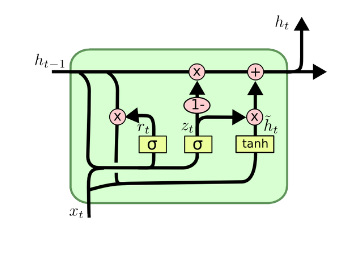
\includegraphics[scale=0.8]{monography/img/models/GRU.png}
    \label{figure:gru}
    \caption[Representação da arquitetura de uma GRU]{Representação da arquitetura de uma GRU\footnotemark}
\end{figure}

Assim como o \textit{\acrshort{LSTM}}, o \acrshort{GRU} também faz uso de mecanismos chamados de Portas que possibilitam que a informação seja atualizada, ou esquecida ao ser transferida de uma célula para outra. Consequentemente, \textit{\acrshort{GRU}} também é capaz de guardar informações importantes na rede de maneira mais eficaz que uma \textit{\acrshort{RNN}} comum. Apesar de parecidos, \textit{\acrshort{GRU}} possui apenas a \textit{Hidden Layer} e duas Portas. Sendo elas as Portas de Atualização e a Porta de Reinicialização. Essas são usadas para fazer o tratamento da informação para simular o efeito de memória, de forma mais específica:

\begin{itemize}
    \item Porta da reinicialização:A porta de reinicialização decide quanto da informação vinda das células passadas será esquecido. E da mesmo forma, caso o valor se aproxime de 0, a informação será esquecida e conforme se aproxima de 1 o valor se mantém.

    \item Porta da atualização: A porta de atualização tem um papel semelhante às Portas de Entrada e Porta de Esquecimento do \textit{\acrshort{LSTM}} . Nela, é decidido quais dos valores provindos das células passadas serão adicionados a rede.
\end{itemize}

Desta forma, nós que aprendem a captura informações de curto-prazo vão ter a Porta de Reinicialização mais ativa e nós que aprendem a captura de informações a longo-prazo vão ter a Porta de Atualização mais ativa \cite{cho2014}. Também vale notar que por ter uma arquitetura mais simples que uma \textit{\acrshort{LSTM}}, o \textit{\acrshort{GRU}} precisa de menos tempo para ser treinado e, geralmente, de menos dados também.
